\documentclass[12pt]{report}
\usepackage[utf8]{inputenc} % and not inputence
\usepackage[T1]{fontenc} % [T1]
\usepackage{lmodern}
\usepackage[swedish]{babel}
\usepackage{hyperref}
\usepackage{graphicx}
\usepackage{caption}


\title{Thesis specification:\\ Semantic parsing of Swedish laws }
\author{
        Mikael Falgard\\ \\
        Provider of the project: Magnus Svernlöv, Notisum AB\\
        Supervisor: Sten Andersson, CSC - KTH\\
        Examiner: Anders Lansner \\\\\\
        \it{Computer Science}\\
        Royal Institute of Technology
        }
\date{\today}


\begin{document}
\maketitle
\section*{Problem}
Rättsnätet is a web service provided by Notisum AB that provides legal information.\footnote[1]{Rättsnätet provides all Swedish laws and Swedish legal cases include preparatory work, government regulations and other legal information from Swedish and European legal sources.} The content on Rättsnätet consists of information gathered from public government databases and has been processed in several steps from plain text to a rich XML file.\\\\
The steps in the process of loading, parsing, analyzing and transforming the information is internally called the Publishing Platform (PP). The PP is a collection of programs written in Delphi, Pascal and C\#. These programs are old and difficult to maintain. Furthermore the conversion parts of the programs are constructed with a conventional technique similar to that used to write compilers. \\
Another public website that also provides legal information, \url{www.lagen.nu}, uses regular expressions when parsing and analyzing the information instead of compiler technology. The corresponding conversions are written in object-oriented Python. Additionally lagen.nu uses a document model from the Semantic Web\footnote[2]{The Semantic Web is a collaborative movement led by the international standards body, the World Wide Web Consortium (W3C). By encouraging the inclusion of semantic content in web pages, the Semantic Web aims at converting the current web dominated by unstructured and semi-structured documents into a web of data.} with the Resource Description Framework (RDF)\footnote[3]{RDF is a general method to decompose any type of knowledge into small pieces, with some rules about the semantics, or meaning, of those pieces. The point is to have a method so simple that it can express any fact, and yet so structured that computer applications can do useful things with it.} as a base. Because of this it has a greater flexibility and follows standards in a better way than Rättsnätet does today.\\\\

\pagebreak

\section*{Goal}
The purpose of the project is to investigate and analyze how Rättsnätet could modernize and replace its current publishing platform to a more modern, easily maintained process based on the RDF model. In addition the processed files should follow the standard that Rättsinformationsprojektet\footnote[4]{Since 1999, authorities producing some kind of legal information are required
to publish it on the internet. However there is no regulation in how those publications should look like. In 2006 this project was launched to further develop the legal information system. \href{http://dev.lagrummet.se/dokumentation/}{Read more at http://dev.lagrummet.se/dokumentation/}} has proposed. The goal is to have a functioning prototype for the parsing stage, that is relatively easy to connect to the existing preprocess (downloading) and post-process (generating HTML). \\\\
There are several issues to have in mind that might complicate the project: 
\begin{itemize} 
\item The amount of documents. There is over 200,000 documents, that amount requires a very fast process. Today the PP does its job in 14 hours a day, but then it only handles a tenth of the documents per day. 
\item Legal source text contains references that should be interpreted differently depending on the context, and to be marked up automatically with a certain margin of error.
\item Cross-references between the 200,000+ documents require theoretically, an array of 40 billion nodes.
\item The output from the process needs to be structurally similar to the current process output so the post process can be used with as little tweaking as possible.\\\\
\end{itemize}

\pagebreak

\section*{Method}
I need to analyze the current process to understand (1) How the process works today. (2) How the output from the process is structured to satisfy the post process. I will read and research (see the Litterature section) the technologies and standards suggested above, Python, regular expression, RDF and XML to get a deeper understanding of them and decide if they are suitable for the task.\\\\
A project like this where the context is very important will also require somewhat understanding of Swedish legal documents. For example it is crucial to understand how a law is structured.\\\\ 
To show that the suggested process works and is fast enough I will develop a prototype that handles SFS data.\footnote[5]{The Swedish Code of Statutes or Svensk författningssamling (SFS) is the official publication of all Swedish laws enacted by the Riksdag and ordinances issued by the Government.} The prototype should be as generic as possible to make it easy to implement parsing of data from other sources later on. Lagen.nu has published its source code as open source, and encurage sharing and reuse of it.\footnote[6]{It is an individual with voluntary interest in the field that drives the development. He is also involved in Rättsinformationsprojektet, and encourages a more structured legal information system.} It is not very well documented (or commented) but should be helpful during the implementation stage. 

\subsubsection*{Limitations}
To make this project feasible it is limited to handling only SFS data. Other types of data sources that a complete process would need to handle are for example:
\begin{itemize}
\item Propositions
\item Supreme Court summaries
\item Decisions of the Courts of Appeal, and the Labour Court
\item European legal regulations and directives\\\\
\end{itemize}


\section*{Litterature}
I have divided the litterature I am going to read into three parts that reflect the different subjects that I will need to research. Furthermore I will take part in Python meetups\footnote[7]{\url{http://www.meetup.com/pysthlm/}} during the year to learn about interesting new technologies, libraries and standards. 
\subsubsection*{Legal information}
\href{http://62.95.69.15/}{Regeringskansliets databases}\footnote[8]{Note that all these litterature references are links.}
\\
\href{http://dev.lagrummet.se/dokumentation/model.pdf}{Document model standard}\\
\href{http://dev.lagrummet.se/dokumentation/introduktion/intro-implementatorer.pdf}{Document model for developers and implementers}\\
\href{http://www.lagrummet.se/Om-lagrummetse/om_lagrummet_se/rattsinformationsprojektet/}{Rättsinformationsprojektet}

\subsubsection*{Semantic Web}
On or more of these books regarding \href{http://www.adlibris.com/se/searchresult.aspx?search=quickfirstpage&quickvalue=semantic+web&title=semantic+web&fromproduct=False}{Semantic Web}\\
\href{http://semanticweb.org/wiki/Semantic_Web_standards}{Semantic Web Standards}\\
\href{http://www.rdfabout.com/quickintro.xpd}{RDF Intro}

\subsubsection*{Code}
\href{http://effbot.org/zone/unicode-objects.htm}{Unicode in Python}\\
\href{http://gnosis.cx/TPiP/}{Text Processing in Python, Chapter 4}\\
\href{http://python.net/~goodger/projects/pycon/2007/idiomatic/handout.html}{Code like a Pythonista}\\
\href{http://www.diveintopython.net/toc/index.html}{Dive into Python}\\\\

\pagebreak

\section*{Timetable}
As the table below shows some of the activites will overlap during the work. I think it might be a good idea to get started on the report as I work on the implementation. This way I can document the source code and design as I go, and I won't have to do it all in the end.\\\\
\begin{tabular}{l l l l}
Description & Start date & End date & Time\\
Project specification, timetable & 1 Aug 2012 & 1 Sep 2012 & (4 weeks) \\
Research, reading litterature & 15 Aug 2012 & 1 Oct 2012 & (6 weeks) \\
Implementation (setting up, testing) & 15 Sep 2012 & 15 Nov 2012 & (8 weeks)\\
Report draft & 1 Oct 2012 & 1 Dec 2012 & (8 weeks)\\
Presentation & 1 Dec 2012 & 15 Dec 2012 & (2 weeks)\\
Finalize report & 15 Dec 2012 & 15 Jan 2013 & (4 weeks)\\
\end{tabular}
\vspace{10pt}

\begin{center}
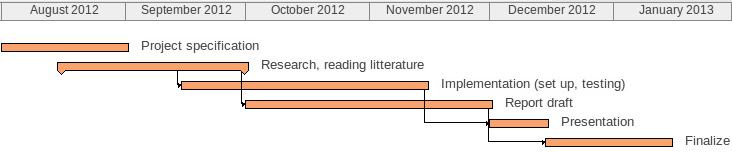
\includegraphics[scale=0.55]{gantt.png}
\captionof{figure}{Gantt chart of the timetable}
\end{center}

\section*{Contact}
Mikael Falgard\\\\
\begin{tabular}{l l}
Persnr & 861031-0156 \\
Email & \href{mailto:falgard@kth.se}{falgard@kth.se} \\
Phone & 070-467 31 34 \\
\end{tabular}\\\\\\
Magnus Svernlöv, Notisum AB \href{mailto:ms@notisum.se}{ms@notisum.se}\\
Sten Andersson, CSC, KTH \href{mailto:stene@csc.kth.se}{stene@csc.kth.se}


\end{document}
